\documentclass[12pt]{article}


\usepackage[english]{babel}
\usepackage{newtxtext} % Times-like font
\usepackage{longtable}

\usepackage{csquotes}
\usepackage[T1]{fontenc} 
\usepackage[a4paper]{geometry}
\usepackage{parskip}
\usepackage{textcomp}
\usepackage{esvect}

\usepackage{pdfpages}

\usepackage{bm}
\usepackage{pdflscape}
\usepackage{booktabs}
\usepackage{amsmath}
\usepackage{multirow}
\usepackage{tikz}
\usepackage{graphicx}% Pictures
\usepackage{amsmath}% to set nice equations
\usepackage{amssymb}% math symbols
\usepackage[hidelinks]{hyperref} %clickable references without colors
\setlength{\parindent}{20pt}
%\usepackage{subcaption}
\usepackage{geometry}
 \geometry{ 
 a4paper,
 left=30mm,
 top=30mm,
 right=30mm,
 bottom=30mm,
 }
\usepackage{subfiles} %Sub files
\usepackage{subfig}%two figures side by side
\usepackage[font=small,labelfont=bf]{caption}
\usepackage{float} %Place floatss
\usepackage{chngcntr}%Changes counter
% \counterwithin{figure}{section} %Set figure counter to section.figure
\usepackage{siunitx} %to put units more easily
\usepackage{calc}

\usepackage{fancyhdr}
\setlength{\headheight}{14.5pt}  % Set headheight to at least 14.49998pt
\pagestyle{fancy}
\usepackage{multirow}
\usepackage{wrapfig}%Posar imatges als laterals
%\usepackage{appendix} %Posa l'apendix a l'índex
\usepackage{afterpage}
\usepackage{color}
\usepackage{listings}
\usepackage{color} %red, green, blue, yellow, cyan, magenta, black, white
\definecolor{mygreen}{RGB}{28,172,0} % color values Red, Green, Blue
\definecolor{mylilas}{RGB}{170,55,241}
%\providecommand{\abs}[1]{\lvert#1\rvert}
%\providecommand{\norm}[1]{\lVert#1\rVert}
\usepackage{eurosym}
\usepackage[natbib=true,
style=ieee,sorting=none]{biblatex}
\addbibresource{References.bib}
\usepackage{indentfirst}
\usepackage{mathtools}
%\usepackage[toc,page]{appendix}
\usepackage{environ}         % provides \BODY
\usepackage{etoolbox}        % provides \ifdimcomp
\usepackage{enumitem}
\hypersetup{   
    urlcolor=cyan,
}
\urlstyle{same}

\newlength{\myl}
\let\origequation=\equation
\let\origendequation=\endequation

\RenewEnviron{equation}{
  \settowidth{\myl}{$\BODY$}                       % calculate width and save as \myl
  \origequation
  \ifdimcomp{\the\linewidth}{>}{\the\myl}
  {\ensuremath{\BODY}}                             % True
  {\resizebox{\linewidth}{!}{\ensuremath{\BODY}}}  % False
  \origendequation
}
\definecolor{mygreen}{rgb}{0,0.6,0}
\definecolor{mygray}{rgb}{0.5,0.5,0.5}
\definecolor{mymauve}{rgb}{0.58,0,0.82}

% Define colors
\definecolor{BlauClar}{RGB}{240, 248, 255}
\definecolor{BlauFort}{RGB}{70, 130, 180}

\usepackage[vlined]{algorithm2e}

\usepackage{tcolorbox}

\lstset{
  backgroundcolor=\color{white},   % choose the background color; you must add \usepackage{color} or \usepackage{xcolor}; should come as last argument
  basicstyle=\footnotesize,        % the size of the fonts that are used for the code
  breakatwhitespace=false,         % sets if automatic breaks should only happen at whitespace
  breaklines=true,                 % sets automatic line breaking
  captionpos=b,                    % sets the caption-position to bottom
  commentstyle=\color{mygreen},    % comment style
  deletekeywords={...},            % if you want to delete keywords from the given language
  escapeinside={\%*}{*)},          % if you want to add LaTeX within your code
  extendedchars=true,              % lets you use non-ASCII characters; for 8-bits encodings only, does not work with UTF-8
  firstnumber=1,                % start line enumeration with line 1000
  frame=single,	                   % adds a frame around the codes
  keepspaces=true,                 % keeps spaces in text, useful for keeping indentation of code (possibly needs columns=flexible)
  keywordstyle=\color{blue},       % keyword style
  language=Matlab,                 % the language of the code
  morekeywords={*,...},            % if you want to add more keywords to the set
  numbers=left,                    % where to put the line-numbers; possible values are (none, left, right)
  numbersep=5pt,                   % how far the line-numbers are from the code
  numberstyle=\tiny\color{mygray}, % the style that is used for the line-numbers
  rulecolor=\color{black},         % if not set, the frame-color may be changed on line-breaks within not-black text (e.g. comments (green here))
  showspaces=false,                % show spaces everywhere adding particular underscores; it overrides 'showstringspaces'
  showstringspaces=false,          % underline spaces within strings only
  showtabs=false,                  % show tabs within strings adding particular underscores
  stepnumber=1,                    % the step between two line-numbers. If it's 1, each line will be numbered
  stringstyle=\color{mymauve},     % string literal style
  tabsize=2,	                   % sets default tabsize to 2 spaces
  %title=\lstname                   % show the filename of files included with \lstinputlisting; also try captions  instead of title
  inputencoding=utf8
}

\lstset{literate=
    {á}{{\'a}}1 {é}{{\'e}}1 {í}{{\'i}}1 {ó}{{\'o}}1 {ú}{{\'u}}1
    {Á}{{\'A}}1 {É}{{\'E}}1 {Í}{{\'I}}1 {Ó}{{\'O}}1 {Ú}{{\'U}}1
    {à}{{\`a}}1 {è}{{\`e}}1 {ì}{{\`i}}1 {ò}{{\`o}}1 {ù}{{\`u}}1
    {À}{{\`A}}1 {È}{{\'E}}1 {Ì}{{\`I}}1 {Ò}{{\`O}}1 {Ù}{{\`U}}1
    {ä}{{\"a}}1 {ë}{{\"e}}1 {ï}{{\"i}}1 {ö}{{\"o}}1 {ü}{{\"u}}1
    {Ä}{{\"A}}1 {Ë}{{\"E}}1 {Ï}{{\"I}}1 {Ö}{{\"O}}1 {Ü}{{\"U}}1
    {â}{{\^a}}1 {ê}{{\^e}}1 {î}{{\^i}}1 {ô}{{\^o}}1 {û}{{\^u}}1
    {Â}{{\^A}}1 {Ê}{{\^E}}1 {Î}{{\^I}}1 {Ô}{{\^O}}1 {Û}{{\^U}}1
    {œ}{{\oe}}1 {Œ}{{\OE}}1 {æ}{{\ae}}1 {Æ}{{\AE}}1 {ß}{{\ss}}1
    {ç}{{\c c}}1 {Ç}{{\c C}}1 {ø}{{\o}}1 {å}{{\r a}}1 {Å}{{\r A}}1
    {€}{{\EUR}}1 {£}{{\pounds}}1
} 

% Sangrado de los párrafos
\setlength{\parindent}{0em}
% Separación entre párrafos
\setlength{\parskip}{3mm}
% Interlineado
\renewcommand{\baselinestretch}{1}


% Hyperref
\definecolor{azulUPC}{RGB}{0, 122, 194} % El color azul de la UPC
\definecolor{azul_titulo}{RGB}{54, 95, 145} % El color azul para los títulos
\usepackage{hyperref}
\hypersetup{
    colorlinks=true,
    citecolor=black,
    linkcolor=black,
    urlcolor=black
}

\usepackage{setspace}
\usepackage[page]{appendix}
\pagestyle{fancy}
\usepackage{nomencl}
\usepackage{booktabs}
\usepackage[export]{adjustbox}

\usepackage{mathrsfs}
\usepackage{fontawesome}
\usepackage{listings}

\newcommand{\ke}{$k-\varepsilon$\,\,\,}
\newcommand{\kw}{$k-\omega$ $SST$\,\,\,}

\newcommand{\etal}{\textit{et al. }}
\makenomenclature

\renewcommand{\nomname}{Nomenclature}

\renewcommand{\nompreamble}{The next list describes several symbols that will be later used within the body of the document}

\begin{document}

{  \makeatletter
    \centering\Large\singlespacing%
    \pagestyle{empty}%
    \begin{figure}[H]
    \centering
    
\includegraphics[width=0.3\linewidth]{Figures/CULogo.png}
    \label{fig:lOGO}
\end{figure}

    \par
    Wahyu Widhi Dyatmika\par
    \vfill
    Towards the Application of Generalised Richardson Extrapolation in Spanwise Oscillating Wall Flow Control Analysis\par
    \vfill%
    SCHOOL OF~\MakeUppercase{AEROSPACE, TRANSPORT AND
MANUFACTURING}\\%
    Computational Fluid Dynamics\par%
    \vfill
    MSc\\
     Academic Year: 2023 - 2024\par
   \vfill
   Supervisor: Tamás Jozsa\\%
   25th August 2023\par
    \vfill\null\cleardoublepage
    \centering\Large%
    \pagestyle{empty}
    \begin{figure}[H]
    \centering
    
\includegraphics[width=0.3\linewidth]{Figures/CULogo.png}
    \label{fig:culogo}
\end{figure}
\par
    \vfill%
    SCHOOL OF~\MakeUppercase{AEROSPACE, TRANSPORT AND
MANUFACTURING}\\%
    Computational Fluid Dynamics\par%
    \vfill
    MSc\par%
    \vfill
    Academic Year: 2023 - 2024\par%
    \vfill
    Wahyu Widhi Dyatmika\par
    \vfill
    Towards the Application of Generalised Richardson Extrapolation in Spanwise Oscillating Wall Flow Control Analysis\par
    \vfill
    Supervisor: Tamás Jozsa\\
     25th August 2024\par
     \vfill
     This thesis is submitted in partial fulfilment of the requirements for the degree of MSc\\%
     \vfill
     \copyright\ Cranfield University 2024. All rights reserved.
    No part of this publication may be reproduced without the written
     permission of the copyright owner.
    \cleardoublepage
    \makeatother
}


\clearpage
\pagestyle{plain}
\pagestyle{fancy}
\fancyhead[R]{} 
\fancyhead[L]{}
\clearpage

\spacing{1.2}
\pagenumbering{Roman}


\section*{Academic Integrity Declaration}

I declare that:

\begin{itemize}
  \item  the thesis submitted has been written by me alone.
  \item  the thesis submitted has not been previously submitted to this university or any
other.
\item  that all content, including primary and/or secondary data, is true to the best of my
knowledge.
\item  that all quotations and references have been duly acknowledged according to the
requirements of academic research.
\end{itemize} 

I understand that to knowingly submit work in violation of the above statement will be
considered by examiners as academic misconduct.



\clearpage
\pagestyle{plain}
\pagestyle{fancy}
\fancyhead[R]{ABSTRACT} 
\fancyhead[L]{}
\clearpage

\spacing{1.2}
\pagenumbering{Roman}


\section*{Abstract}




\clearpage
\pagestyle{plain}
\pagestyle{fancy}
\fancyhead[R]{ACKNOWLEDGEMENT} 
\fancyhead[L]{}
\clearpage

\spacing{1.2}
\pagenumbering{Roman}


\section*{Acknowledgement}






%\addtocontents{toc}{\protect\thispagestyle{empty}} % for the first page
\clearpage
{
  \hypersetup{linkcolor=black}
  \pagestyle{fancy}
    \fancyhead[R]{TABLE OF CONTENTS} 
    \fancyhead[L]{}
  \tableofcontents
  \clearpage
    \pagestyle{fancy}
    \fancyhead[R]{LIST OF FIGURES} 
    \fancyhead[L]{}
  \addcontentsline{toc}{section}{List of figures}
  \listoffigures
  \clearpage
    \pagestyle{fancy}
    \fancyhead[R]{LIST OF TABLES} 
    \fancyhead[L]{}
  \addcontentsline{toc}{section}{List of tables}
  \listoftables
}

%\clearpage


%\clearpage
%\nomenclature{EFD}{Experimental Fluid Dynamics}
%%\nomenclature{CFD}{Computational Fluid Dynamics}
%\nomenclature{CRWTs}{Common Research Wind Tunnels}
%\nomenclature{RANS}{Reynolds-averaged Navier-Stokes }





%\addcontentsline{toc}{section}{Nomenclature}
%\printnomenclature
%\setlength{\parskip}{0.5cm}



\newpage
\pagenumbering{arabic}
\setcounter{page}{1}


\sloppy
\pagestyle{fancy}
\lhead{\small{}}
\rhead{{\small{LIST OF SYMBOLS AND ABBREVIATIONS}}}

\section*{List of Symbols and Abbreviations}
\begin{tabbing}
	\textbf{Abbreviations} \= \\
	CFD \> Computational Fluid Dynamics\\
	CF \> Channel Flow \\
	DNS \> Direct Numerical Simulation \\
	GREP \> Generalised Richardson Extrapolation \\
	ISA \> Inner-Scale Actuation \\
	LES \> Large-Eddy Simulation\\
	NPS \> Net Power Saving \\
	NR \> Normalised Resolution \\
	OSA \> Outer-Scale Actuation\\
	PF \> Pipe Flow \\
	RANS \> Reynolds Averaged Navier Stokes\\
	\\
	\textbf{Variables (Latin Letters)}\\
	E \> Energy\\
	\textbf{e} \> Vector component \\
	\textbf{g} \> Gravitational vector \\
	h \> Height \\
	$L_o$ \> Integral Length Scale\\
	n \> Variable for showing time step \\
	P \> Pressure \\
	Re \> Reynolds number\\
	t \> Time \\
	\textbf{u} \> Velocity vector \\
	$u$. $v$, $w$ \> Streamwise, wall-normal, and spanwise velocity, respectively\\
	$x$, $y$, $z$  \> Streamwise, wall-normal and spanwise direction, respectively\\
	\\
	
	\textbf{Variables (Greek Letters)}\\
	$\delta$ \> Characteristic length \\
	$\eta$ \> Kolmogorov length scale\\
	$\kappa$ \> Wave number \\
	$\lambda$ \> Minimal flow length \\
	$\nu$ \> Kinematic viscosity \\
	$\mu$ \> Dynamic viscosity\\
	$\rho$ \> Density\\
	$\phi$ \> Transported quantity
	\\
	\\
	\textbf{Subscripts and Superscripts}\\
	$*$ \> Intermediate values\\
	$+$ \> Wall-normal value\\
	$\tau$ \> Viscous quantities
	
\end{tabbing}









%\nocite{*}
\clearpage
\pagestyle{fancy}
\lhead{\small{}}
\rhead{{\small{1. INTRODUCTION}}}
%\vspace{-2cm}
\section{Introduction} 
\label{sec:intro}
In the subject of fluid dynamics, flow control can massively influence the performance of the flow around or inside an object. Designing a flow control method requires intricate understanding of flow behaviours such as dynamics and turbulence. Designing a proper flow control can be essential for maximising the efficiency of the system.


\subsection{Motivation}
\label{sec:motivation}
Climate change has been a driving factor for engineering design in the modern world \cite{Douglas2017}. The changes in climate pattern has proven to be detrimental to human and other living being. One of the causes of the climate change is the emission of energy generation process, such as carbon dioxide \cite{Met_Officend}. However, the need of creating more energy is indispensable as human population grows continuously, with energy requirement predicted to reach more than the triple of global energy requirement today \cite{IRENA2023}. This requires engineers to create a high performance solution with a consideration of efficiency in its operations. In aerospace sector, this approach is also used as the sector creates 2\% of the total global emission, which is the largest among other means of transportation \cite{Iea2023}. Generally in aerospace sector, high efficiency value can be reached by minimising drag, which generated from the viscous drag, as shown in Figure \ref{fig:B737}.
The viscous drag can be practically reduced in a controlled manner using flow control strategies, offers a solution for a sustainable aerospace future \cite{Abbas2017}.

\begin{figure}[ht]
    \centering
    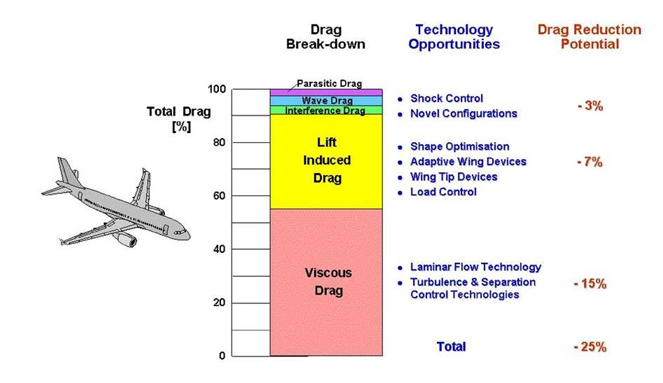
\includegraphics[width=0.75\linewidth]{Figures/B737Drag.png}
    \caption{Drag and Reduction Potential in a General Aircraft~\cite{Abbas2017}}
    \label{fig:B737}
\end{figure}


Fluid flow control has been a major topic in fluid dynamics. Fluid flow control strategies have been implemented in various areas, such as aerospace, wind energy sector, industrial process designs, and water management \cite{Airiau2016}. The development of flow control methods was born from the understanding of the presence of turbulence in a fluid flow. Turbulence in a moving flow can generally be denoted by the chaotic behaviour of the fluid \cite{Benzi2023}, typically in the form of eddies or vortices. The interaction of the flow with itself, along with the solid object nearby can produce drag, which reduces the flow velocity and its ability to transport its properties \cite{Bell1979}. In most systems, the drag can be detrimental as it can reduce the efficiency of the system. Because of that, flow control strategies are introduced to force the fluid to move in a regulated behaviour to decrease the drag produced in the system. 

Currently, multiple strategies and approaches towards an efficient flow control system are studied. One of recent studies \cite{Marusic2021} suggests that an active flow control strategy in the form of spanwise wall oscillations can generate a positive net power saving value for high Reynolds number regimes. With the finding, a pathway for an industrial-wide application of oscillating wall flow control can be opened and hence a further studies are needed.

In order to further expand the spanwise wall oscillation flow control strategy, understanding the turbulence in the flow is of utmost importance, especially in the near wall region. Turbulence is the chaotic nature of a fluid flow, caused by "a complex interplay of multiple flow patterns occurring simultaneously, making difficult to model and predict accurately" \cite{Alberti2023}. Therefore, intricate physics modelling is generally required to completely simulate the turbulence in the flow, which growingly expensive in terms of computational cost as the Reynolds number increases \cite{Chen2021}. In this paper, ensemble averaging is introduced as a solution for simulating intricate turbulence in a spanwise oscillating wall flow control analysis.



\subsection{Literature  Review}

\subsubsection{Physics of Wall Bounded Flow Turbulence}
\label{sec:litrev_oscwall}
Turbulence can be defined as the swirling motion that happened randomly in the fluid flow \cite{Sreenivasan1999}. Due to its randomness, turbulence phenomena can sometimes be too complicated and difficult to comprehend \cite{Hussain1986}. Therefore, most turbulence studies are focused on understanding the coherent structures, which are the regions with recognisable concentrated vorticity \cite{Fiedler1988}. As seen in Figure \ref{fig:hairpintamas}, there are common structures in the flow region near the wall that is identifiable. The most prominent structure is the hairpin vortex, which indicated by a raising arch head with two streamwise-oriented legs \cite{Wang2015}.
\pagebreak
\begin{figure}[ht]
    \centering
    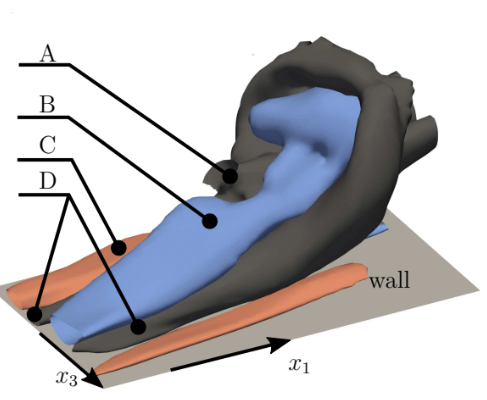
\includegraphics[width=0.5\linewidth]{Figures/Hairpin2.png}
    \caption{Near Wall Coherent Structures: A) Hairpin Vortex ; B) Low momentum region; C) high momentum region; D) counter-rotating quasi-streamwise vortices~\cite{Tamas2019}}
    \label{fig:hairpintamas}
\end{figure}

Several researches, such as the studies made by Wang \cite{Wang2015} and Alfonsi \cite{Alfonsi2006} explained how the hairpin vortices generated. First, the legs of the hairpin vortices, which consist of two quasi-streamline, counter-rotating vortices are interacted with each other. These vortices rises to the area with lower shear magnitudes, which decreases the vorticity magnitude. With the opposing rotational direction, the coalescence of two vortical structures are occurred and the hairpin vortices are generated. Inside the vortex, low momentum region is generated. Conversely, the high momentum region is generated outside the two counter-rotating vortices.

Other than the physical structures, the spectral analysis is also commonly conducted to understand the turbulence phenomena. Generally, spectral analysis involves analysing the turbulence through the wave energy distribution in the structures \cite{Fan2023}. In order to visualise the energy distribution, the Kolmogorov spectrum is used, as shown in the Figure \ref{fig:specturb}.

Based on Brennen \cite{Brennen2004}, there are 3 main regions in the spectrum. The first is the integral region, or commonly known as the energy containing range. This characterises the overall size of the largest eddies, which contains the energy in the flow. These large scale structures are responsible for transfering energy to the from the external forces to the smaller structures in the turbulent flow. The energy is then cascades to the smaller scales through the inertial region. The energy spectrum in this region follows a power law distribution:
\begin{equation}
    E(k) \propto k^{\frac53}
\end{equation}
Where k is wave number. Afterwards, the energy cascades to the smallest scales, which are in the Kolmogorov scales. In this scales, the viscosity dominates and the kinetic energy is transfered to heat energy.

\begin{figure}
    \centering
    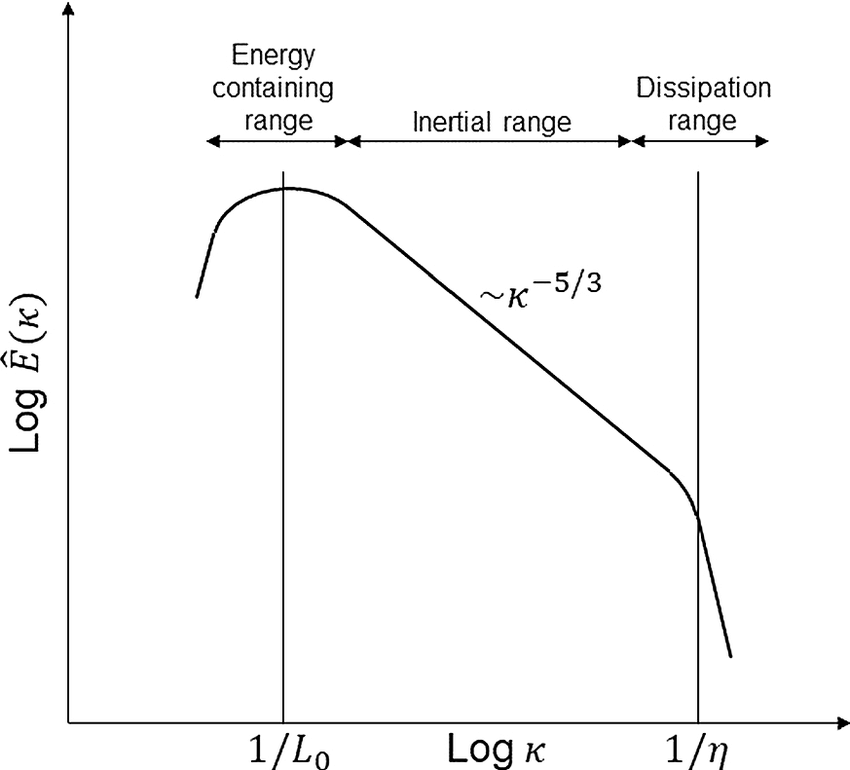
\includegraphics[width=0.65\linewidth]{Figures/KolmogorovSpectrum.png}
    \caption{Typical Energy Spectrum in a Flow ~\cite{kalmar-Nagy2019}}
    \label{fig:specturb}
\end{figure}

%Dont understand about hairpin, Add about spectral??



\subsubsection{Spanwise Oscillating Wall Flow Control}
\label{sec:litrev_oscwallfc}
Flow control can be defined as the method of altering the flow to a desired state or path \cite{Jahamiri2010}. Typically, there are two types of flow control methods, as stated by Ricco \cite{Ricco2021}. The first method is the passive flow control, which requires no actuation or movement in the system, thus no external energy required to control the fluid flow. The second method is the active flow control. Contrary to its passive counterpart, the active flow control requires energy to actuate a motion in a flow. 

Due to the certain energy consumption, most of the study regarding active flow control are circulated around the strategy to create a motion that has a positive net power saving. The same trend has been observed for spanwise oscillating wall method, which requires actuation to create an oscillation in the near wall region. The concepts and methods are documented in Table \ref{tab:studies_spowfc}. 

\pagebreak
\begin{landscape}
\begin{longtable}{@{}lllll@{}}
\caption{Experimental and Computational Studies of Spanwise Oscillating Wall Flow Control}
\label{tab:studies_spowfc}\\
\hline
\multicolumn{1}{c}{\textbf{References}} & \multicolumn{1}{c}{\textbf{Geometry}} & \multicolumn{1}{c}{\textbf{Methodology}} & \textbf{Reynolds Number} & \textbf{NPS$_{max}$ ($\%$)} \\ \hline
\endfirsthead
%
\endhead
%
\hline
\endfoot
%
\endlastfoot
%
Marusic et al. (2021) \cite{Marusic2021} & CF & \begin{tabular}[t]{@{}l@{}}Experimental: Hot-wire \\ anemometry\\ Computational: LES (dynamic \\ Smagorinsky)\end{tabular} & \begin{tabular}[t]{@{}l@{}}Re$_\tau$ = 6000\\ Re$_\tau$ = 12800\end{tabular} & \begin{tabular}[t]{@{}l@{}}$\sim$7\\ $\sim$2\end{tabular} \\
Gatti and Quadrio (2016) \cite{Gatti2016} & CF & Computational: DNS & \begin{tabular}[t]{@{}l@{}}Re$_\tau$ = 200\\ Re$_\tau$ = 1000\end{tabular} & \begin{tabular}[t]{@{}l@{}}5.3 $\pm$ 0.24\\ 3.9 $\pm$ 0.31\end{tabular} \\
Quadrio et al. \cite{Quadrio2009} & CF & Computational: DNS & Re = 4760 & 5 \\
Auteri et al. (2010) \cite{Auteri2010} & PF & \begin{tabular}[t]{@{}l@{}}Experimental, with DNS \\ comparison from \cite{Quadrio2009}\end{tabular} & Re = 4760 & 17 \\
Viotti et al. (2009) \cite{Viotti2009} & CF & Computational: DNS & Re$_\tau$ = 200 & 23 \\
Chandran et al. (2023) \cite{Chandran2023} & CF & \begin{tabular}[t]{@{}l@{}}Experimental: Drag Balance and \\ Hot Wire Anemometry\end{tabular} & 4500 $\leq$ Re$_\tau$ $\leq$ 150000 & \begin{tabular}[t]{@{}l@{}}ISA: -40\\ OSA: 5-10\end{tabular} \\
Deshpande et al. (2024) \cite{Deshpande2024} & CF & Computational: DNS & Re$_\tau$ $\approx$ 300 & Not reported \\
Nguyen et al. (2021) \cite{Nguyen2021} & CF (with square bar) & Computational: DNS & Re$_\tau$ = 218 & 0.8 \\
Ricco et al. (2012) \cite{Ricco2012} & CF (rough wall) & Computational: DNS & Re$_\tau$ = 200 & Not reported \\ \hline
\end{longtable}

\end{landscape}

The key trend from the results is the NPS value is dependent from various factors. It is apparent from the studies that the NPS value of of the flow control decreases as the Reynolds number increases \cite{Gatti2016} \cite{Quadrio2009}. Other than that, the net power saving also relies on the wave function applied. From the studies, it can be seen that the net power saving is positive when the wave function of the oscillating wall matches the large-scale eddies inside the flow \cite{Marusic2021}\cite{Chandran2023}.

Based on the table, a simple channel flow is the most common base case to test the effectivity of flow control. This is due to the simplicity of the flow modelling as the case only has two wall surface, generally placed on the top and the bottom of the domain. The domain surfaces on the side are assumed to be free surfaces \cite{Apsley2023}. To the boundary condition assignment, the effect of the wall in the flow will be easier to analyse without having to take account the wall perpendicular to the wall of interest.

\subsubsection{Turbulence Modelling}
\label{sec:litrev_turbmethod}
Solving turbulence is required in order to create a good model of a fluid flow. This is because turbulence is highly related to the transport of mass, energy, and other values in the flow \cite{Trench2023}. However, variety in the temporal and spatial scale of turbulence oftentimes requires high computational power \cite{Duraisamy2019}. To alleviate the excessive computational power, turbulence modelling is often used, generally in the form of Reynolds Averaged Navier Stokes (RANS) \cite{Sidik2020}. However, due to the nature of the modelling, some simplifications leads to information loss, especially regarding the energy cascade to the small scales \cite{bush2020}. Other approach that can be done is using the Large Eddy Simulation (LES). LES method solves large eddies directly, but uses modelling to solve the small eddies \cite{Zhiyin2015}. This way, high accuracy can be obtained for the large structures, while maintaining low computational expenses. However, similar to RANS modelling, inaccuracy can occur in small-scale turbulence \cite{Mason1994}.

In cases where the effect of small-scales turbulence are heavily considered, turbulence modelling is fully disregarded. This means that the Navier-Stokes equations are directly solved \cite{Moin1998}. These method of solving the fluid flow is termed Direct Numerical Simulation (DNS). Ideally, DNS should be performed with spatial resolution at least as large as the Kolmogorov scale, which the smallest eddies that can be produced by the flow \cite{Boschung2016}. However, the fine grid resolution will make the analysis prohibitively expensive. Therefore, lower resolution usually preferred to DNS methods. %How much?

\subsubsection{Generalised Richardson Extrapolation}
In a computational analysis, the domain settings may change the value of the results. The finer the settings is, the higher the quality of the results. However, finer results require high computational resources which limits the resolution of the model. To counter the problem. the Richardson extrapolation is usually used. Richardson extrapolation can be defined as the approximation of the ideal value of convergent value using \cite{roache2009verification}:
\begin{equation}
	f_{h=0} \stackrel{\sim}{=} \frac43 f_1 - \frac13 f_2
\end{equation}

However, most of the application of Richardson extrapolation are limited to the spatial convergence. The novel method of Richardson extrapolation includes temporal and domain size to determine the best resolution of a computational case. The combined resolution is expressed as:

\begin{equation}
	Normalised Resolution = \frac{\Delta x_e^{current}}{\Delta x_e^{finest}} \frac{\Delta t^{current}}{\Delta t^{finest}} \frac{t_{tot}^{finest}}{t_{tot}^{current}} \frac{L_e^{finest}}{L_e^{current}}
\end{equation}

\subsubsection{Sample Averaging}
To understand the overall trend of a numerical result, the result must be averaged. The averaging is normally done using two different method. First is time averaging, which is the more common practice in CFD analysis. Time averaging involves obtaining the flow properties such as velocities and pressure over a long period of time. After that, the flow value is averaged. This way, the fluctuations during a transient analysis can be avoided, thus making further calculations easier \cite{Kallio2015}. Because of this, the time-averaging method is popular in steady-state analysis \cite{Sodja2007}. However, the long period sampling time requires high computational resources, especially when high-fidelity approaches are used \cite{Makarashvili2016}.

The alternative method of sample averaging is using the ensemble averaging. By definition, ensemble averaging requires "averaging over numerous independent simulations"\cite{Tosi2021}. Ensemble averaging decreases the requirement of computational power, thus making the analysis more efficient, especially in high Reynolds number \cite{Makarashvili2016}. Currently, the method is not popular in fluid dynamics, but the method is commonly used in molecular dynamics, where time-averaging is very costly to perform \cite{Gordiz2015}.

In a practical sense, time and ensemble averaging have a possibility to have the correlating result to one and another. This commonly referred as ergodicity, a statistical property that exhibits that the system has the equal value of ensemble and time averaging \cite{Yamamoto2024}. Turbulent flow, as shown in recent study \cite{Galanti2004}, has known to be ergodic. Therefore, turbulent flow analysis can benefit from both methods without sacrificing the result generation.

\subsubsection{Xcompact3d}
\label{sec:litrev_ic3d}
The research mainly uses Xcompact3d to solve the fluid flow. Xcompact3d is a FORTRAN 90 based open-source software purposed to simulate incompressible fluid flows \cite{Bartholomew2020}. The software uses high order compact schemes \cite{Laizet2014}, which utilises shortened version of high order schemes. This way, the analysis will still satisfy the need of high resolution of high-order schemes, while maintaining simplicity of low-order schemes \cite{Laizet2009}, making the compact schemes a powerful and efficient tool to solve turbulence.

%Choice of the compact schemes
%Workflows

With the higher order schemes, the simulation can run high fidelity schemes to solve the viscous terms in the Navier-Stokes equation. The two models that are available to use in Incompact3d is Large Eddy Simulation (LES) and Direct Numerical Simulation (DNS) \cite{Laizet2014}. As the section \ref{sec:litrev_turbmethod} suggests, both methods are preferable when it comes to analysing turbulence in detail.

%%LES method --> simagorinsky
%%DNS Method???


\subsubsection{Knowledge Gap}
\label{sec:litrev_knowgap}
Current spanwise oscillating wall flow control research lacks a thorough analysis in high Reynolds number. To conduct flow control studies using CFD, researchers must analyse turbulence in great depth, usually using LES or DNS analysis. This leads to high computational expenses. The requirement of high computational power also increased with the increase of Reynolds number. Moreover, the studies conducted uses time--averaged approaches, further pushing the need of ensemble averaging approach as an alternative approach. With this study, future study can hopefully be conducted at a high Reynolds number region that could not be done before.


\subsection{Aim and Objectives}
\label{sec:Aim and objectives}
The aim of the study is to analyse the effectivity of ensemble averaging in numerical analysis of spanwise oscillating wall flow control.

With this aim, the objectives can be set as the steps to achieve the aim set. The objectives are set as follows:
\begin{itemize}[noitemsep]
    \item Generate a channel flow grid as a case for the study
    \item Generate a generalised Richardson extrapolation by changing the spatial and temporal resolution
    \item Conduct flow simulations of the channel flow with and without spanwise oscillating wall flow control using DNS
    \item Generate and compare the time and ensemble averaging results using post-processing methods

\end{itemize}



\subsection{Synopsis}
\label{sec:Sinopsis}
The thesis is arranged to be in a form as follows. Section \ref{sec:Methodology} provides the theoretical background and the methodology for the thesis. The governing equations, along with the supporting equations used in the numerical simulations are thoroughly explained. Moreover, the computational procedures, including geometry and mesh generations, simulations settings and post processing methods are introduced in this section.

Results obtained from the analysis is displayed in Section \ref{sec:Results & Discussion}. The discussion is then served as the rationale of the result. Several figures and tables are displayed as a summary for the result and an aid for understanding the phenomena behind the flow condition. Section \ref{sec:Conclusions & Recommendations} presents the conclusions of the current study and recommendations for future studies.

\clearpage
\pagestyle{fancy}
\lhead{\small{}}
\rhead{{\small{2. METHODOLOGY}}}
\clearpage
\section{Methodology}
\label{sec:Methodology}


%%%%%%%%%%%%%%%%%%%%%%%%%%%%%%%%%%%%%%%%%%%%%%%%%%%%%%%%%%%%%%%%%%%%%%%%%%%%%%%%%%%%%%%%%%%%%%%%%%%%%%%%%%%%%%%%%%%%%%%%%%%%%%%%%%%%%%%%%%%%%%%%%%%%%%%%%%%%%%%%%%%%%%%%%%%%%%%%%%%%%%%%%%%%%%%%%%%%%%%%%%%%%%%%%%%%%%%%%%%%%%%%%%%%%%%%%%%%%%%%%%%%%%%%%%%%%%%%%%%%%%%%%%%%%%%%%%%%%%%%%%%%%%%%%%%%%%%%%%%%%%%%%%%%%%%%%%%%%%%%%%%%%%%%%%%%%%%%%%%%%%%%%%%%%%%%%%%%%%%%

\subsection{Flow Problem of Interest}
\label{sec:Flow problem of interest}
\subsubsection{Cylindrical Flow}
As a test case for running the Xcompact3d, a simple cylindrical wake case is used. In this case, the a cylinder is subjected to a flow that creates a oscillating flow behind that are commonly known as the vortex shedding phenomenon. The parameters of the cylinder is set as default, given by the input example, shown in Table \ref{tab:cyl_wake_case}.

\begin{table}[h!]
	\caption{Cylinder Wake Case Parameters}
	\centering
	\label{tab:cyl_wake_case}
	\begin{tabular}{ccccccc}
		\hline
		Re  & $x_{cyl}$ & $y_{cyl}$ & $r_{cyl}$ & $u_b$ & $\rho$ & $\nu$   \\ \hline
		300 & 5       & 6       & 0.5     & 1     & 1      & 0.0033 \\ \hline
	\end{tabular}
\end{table}

It is worth noting that the cylinder wake case is only used as a means to check the result quality of Xcompact3d case. Therefore, the cylinder wake case will not be analysed as in depth as the channel flow cases.

\subsubsection{Channel Flow}
To understand the effect of oscillating wall flow control to the effect of the flow, a case must be formulated as an example case. Generally, the case used is a canonical flow problem, which the information and data are abundantly accessible and can easily compared to one and another. Therefore, the turbulence phenomena can be thoroughly examined. In this study, a simple double periodic channel flow problem is used to be analysed for the oscillating wall flow control problem. Double periodic channel flow cases utilises periodic boundary conditions on two sets of planes: spanwise and streamwise planes. 

The first thing to do when simulating a double periodic channel flow problem is to determine the requirement of the channel flow domain size. The size of the domain must be meticulously determined to minimise the computational expenses but ensuring all of the necessary turbulence structures are captured appropriately. The minimum size of the double periodic channel flows are commonly referred as the minimal flow unit \cite{Jimenez1991}, shown in Figure \ref{fig:jimenezmfu}.

\begin{figure}[ht]
	\centering
	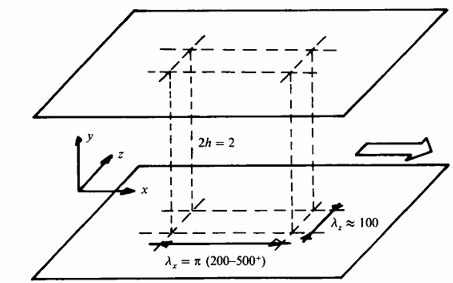
\includegraphics[width=0.6\linewidth]{Figures/JimenezMFU}
	\caption{Minimal Flow Unit of a Double Periodic Channel Flow~\cite{Jimenez1991}}
	\label{fig:jimenezmfu}
\end{figure}

\pagebreak
The length of the minimal flow unit is defined in a wall flow unit, denoted by the (+) sign. The (+) sign is a normalisation of quantities using the viscous length scale, formulated as:

\begin{equation}
	\delta_\nu = \frac{\nu}{u_\tau}
\end{equation}

Where $u_\tau$ is a function of wall friction, defined as \cite{Pope2000}:

\begin{equation}
	u_\tau = \sqrt{\frac{\tau_w}{\rho}}
\end{equation}

$\tau_w$ is related to the Reynolds numbers and the velocity gradient to the normal direction, stated as \cite{Daniel2017}:
\begin{equation}
	\tau_{w} = \frac{\partial u}{\partial y} Re
\end{equation}

$Re$ is the dimensionless number which displays the ratio between the inertial and viscous forces, expressed as \cite{NASA_Re}:
\begin{equation}
	Re = \frac{v \delta}{\nu}
\end{equation}

For study in turbulence, friction Reynolds numbers are more commonly used due to its relevance to the near wall turbulence. The equation of the friction Reynolds number is displayed below \cite{Pope2000}.
\begin{equation}
	Re_\tau = \frac{u_\tau \delta}{\nu} \approx 0.09 (2Re)^{0.88} 
\end{equation}

For the base case, the Reynolds number are defined as $Re_\tau = 180$. The quantity is chosen due to the availability of DNS channel flow data \cite{Lee2015} and the data from Xcompact3D \cite{Bartholomew2020}. The fluid properties data is shown in the Table \ref{tab:fluprop} below.

\begin{table}[ht]
	\caption{Fluid Properties}
	\label{tab:fluprop}
	\centering
	\begin{tabular}{lccccc}
		\hline
		{$\boldsymbol{Re_\tau}$} & {Re} & {$\boldsymbol{u_b}$} & {$\boldsymbol{\rho}$} & {$\boldsymbol{\nu}$} \\ \hline
		180               & 2819.294    & 1          & 1               & 0.00035        \\ \hline
	\end{tabular}
\end{table}
 



\subsection{Theoretical Background}
\label{sec:Governing equations SECTION}




\subsubsection{Governing Equations of Incompressible Fluid Flow}
\label{sec:Governing equations comp}

In a low Reynolds number case such as defined in Section \ref{sec:Flow_prob_interest}, the fluid becomes incompressible, which transforms both governing equations of the fluid flow \cite{Konoszy2024}. For the continuity equation, the expression simplifies into:

\begin{equation}
	\nabla \mathbf{u} = 0
\end{equation}

The bold variables denotes a field. For the context of $\mathbf{u}$, which is the velocity field, it can be expanded into:
\begin{equation}
	\mathbf{u} = u \mathbf{e_x} + v \mathbf{e_y} + w \mathbf{e_z}
\end{equation}

On the other hand, the momentum equation changes by dropping the compressibility term. Moreover, because of no height change involved in the channel flow, the gravity term is also dropped. Additionally, the momentum equation can be modified by normalising every term to density, as density remains constant in incompressible flow.

\begin{equation}
	\underbrace{\frac{\partial \mathbf{u}}{\partial t}}_{\rm I.} + \underbrace{(\mathbf{u}\cdot \nabla)\mathbf{u}}_{\rm II.} = - \underbrace{\frac{1}{\rho}\nabla p}_{\rm III.} + \underbrace{\nu \nabla^2 \mathbf{u}}_{\rm IV.}
\end{equation}

There are four members in a incompressible Navier-Stokes equation. The term I is the unsteady term, showing the change of the fluid velocity over time. The term II is the convective term, showing the transport of properties in the flow. The third term is the pressure gradient, showing the change of pressure in the fluid. Lastly, term IV, determines how the viscous diffusion and dissipation affecting the flow.

\subsubsection{Fractional Step Method}
\label{sec:Frac_step}
In incompressible flow, the density remains constant while the pressure changes. Therefore, the equation of state is not applicable \cite{Konoszy2024}, hence pressure and velocity equation must be calculated together in a coupled equation. In Xcompact3D, the Fractional Step Method is used \cite{Laizet2024}. In Fractional Step method, there are four steps that is conducted to couple the pressure and velocity variables \cite{Westra2002}. The first step utilises intermediate velocity field, which is expressed as \cite{vanKan1986}:
\begin{equation}
	\frac{\hat{\mathbf{u}}^{k} - \mathbf{u}^{k-1}} {\Delta t} = \gamma_{k} \mathcal{A}(\mathbf{u}^{k-1}) + \theta_{k} \mathcal{A}(\mathbf{u}^{k-2}) - \alpha_{k} \nabla p^{k-1}
\end{equation}
Where $\mathcal{A}$ is the convection-diffusion operator, which includes both terms II and IV of the Navier-Stokes equations \cite{Tamas2019}. It also worth noting that the intermediate velocity field does not satisfy the continuity equation due to its divergence-free characteristics.

Then, the second step is to solve the predicted scalar field, using the following relation:
\begin{equation}
	\nabla^2 \phi^{k} = \frac{1}{\alpha_k \Delta t}\nabla{\hat{\mathbf{u}}^k}
\end{equation}
This step is based on the pressure-Poisson equation, which makes this step computationally demanding \cite{Tamas2019}. Therefore, 3D FFT scheme is used to solve the scalar field equation \cite{Li2010}.

The third step is to update the velocity using the known scalar field and intermediate velocity field.
\begin{equation}
	\mathbf{u}^k = \hat{\mathbf{u}}^{k} - \alpha_k \Delta t \nabla \phi^{k}
\end{equation}
Finally, the pressure field is updated using the relation with the scalar field:
\begin{equation}
	p^k = p^{k-1} + \phi^k
\end{equation}


\subsubsection{Spatial Discretisation}
Solving the Navier-Stokes equation numerically requires spatial discretisation, which involves transferring the properties of the flow from one member to another \cite{Hawez2021}. Xcompact3d uses various types of compact finite difference schemes \cite{Laizet2009}, due to its ability to solve the derived values of a defined point and the neighbouring members simultaneously. This study uses the 6th-order centred Hermitian compact scheme, which solved the first derivation of the values as: \cite{Laizet2024UserGuide}:

\begin{equation}
	\alpha \mathbf{u}'_{i-1} + \mathbf{u}'_{i} + \alpha \mathbf{u}'_{i+1} = a \frac{\mathbf{u}_{i+1} - \mathbf{u}_{i-1}}{2 \Delta x} + b \frac{\mathbf{u}_{i+2} - \mathbf{u}_{i-2}}{4 \Delta x}
	\label{eq:6orderHOC}
\end{equation}

For the variables, it is set into $\alpha = 1/3$, $a = 14/9$, and $b = 1/9$ to ensure the scheme can represent a wide range of turbulence scales \cite{Laizet2009}. The second derivative also uses the 6th-order central scheme, expressed as:

\begin{equation}
	\alpha \mathbf{u}''_{j}+ \mathbf{u}''_{j+1} + \alpha \mathbf{u}''_{j+1} = a \frac{\mathbf{u}_{i+1} - 2\mathbf{u}_{i} + \mathbf{u}_{i-1}}{\Delta x^2} + b \frac{\mathbf{u}_{i+2} - 2\mathbf{u}_{i} + \mathbf{u}_{i-2}}{4\Delta x^2} + c \frac{\mathbf{u}_{i+3} - 2\mathbf{u}_{i} + \mathbf{u}_{i-3}}{9\Delta x^2}
	\label{eq:6orderHOC2nddev}
\end{equation}

To ensure the same range as the first derivative, the variables $\alpha$ is set to 2/11,  $a$ is set to 12/11, $b$ is set to 3/11, and $c$ is set to 0. Using these equations and the said variables value, the scheme can calculate the results with 4 or 5 times lower number of mesh nodes compared to 2nd order schemes while only increasing 2 times of its computational expenses \cite{Laizet2024}.




\subsubsection{Temporal Discretisation}
\label{sec:temp_disc}
Other than the spatial discretisation, temporal discretisation must also be applied to calculation so the numerical simulation can be progressed to the next time step. For nearly all of the time discretisation, the third-order Adam-Bashforth equation is used. The third order Adam-Bashforth scheme is an explicit scheme that uses one equation to progress the time step of the calculation \cite{Durran1991}, displayed as:
\begin{equation}
	\phi^{n+1} - \phi^{n} = \frac{\Delta t}{12} [23F^{n} - 16F^{n+1}+5F^{n-2}]
\end{equation}

Where
\begin{equation*}
	\begin{gathered}
		F^n = \mathbf{u}^n \phi^n\\
		F^{n-1} = \mathbf{u}^{n-1} \phi^{n-1}\\
		F^{n-2} = \mathbf{u}^{n-2} \phi^{n-2}\\
		\label{eq:Fhalf}
	\end{gathered}
\end{equation*}

For the diffusion term in the wall-normal direction, the implicit Crank-Nicolson equation is also used for the time discretisation. The temporal discretisation for the y-diffusion term can be expressed as:

\begin{equation}
	\left( \nu \frac{\partial^2 v}{\partial y^2} \right)^{n+\frac{1}{2}} = \frac{1}{2} \left( \nu \frac{\partial^2 v^{n+1}}{\partial y^2} + \nu \frac{\partial^2 v^n}{\partial y^2} \right)
\end{equation}




\subsection{Computational Procedures}
\label{sec:Computational procedures}

\subsubsection{Xcompact3d Setup}
\label{sec:Xcompact3d Setup}
Xcompact3d, as any other FORTRAN F90 based code, must be downloaded and compiled before being able to be used as an analysis software. The code is downloaded through its official Github repository, using:
\begin{verbatim}
	git clone https://github.com/xcompact3d/Incompact3d
\end{verbatim}

After that, the code is compiled using the following commands on unix, assuming 8 threads are available for compiling the code:
\begin{verbatim}
	cd Incompact3d
	export FC=mpif90
	cmake -S . -B build
	cd build
	cmake --build . -j 8
\end{verbatim}

Then by going to the \textit{input.i3d} file in each example code, the boundary conditions, as well as domain size, number of mesh, and initial condition can be changed.

%job script??? what kind of integration do you want?
 

\subsubsection{Grid Generation}
\label{sec:Gridgen}
For the entirety of the study, the cartesian structured grid is used. The entire model is discretised into a system of hexahedral-shaped elements with eight nodes connecting to each other \cite{Yeoh2010}. In a simple canonical flow as this study, the structured hexahedral grid is favoured due to the the efficiency of the shape in terms of filling the spaces, as well as the ability of minimising diffusion when transfering the properties from an element to another \cite{ANSYS2020}. Additionally, the simple connectivity of the elements makes the grid model simple to program \cite{TU2018125}.

To capture the near-wall turbulence, the size of the grid near the wall must be decreased. However, just uniformly decrease the size of the grid may cause an unnecessary computational expense as the flow on the centre of the channel flow do not have substantial gradient or turbulence structures. To compensate the problem, a stretching algorithm is introduced in the Xcompact3d program \cite{Laizet2009}, developed from \cite{Cain1984} and \cite{Avital2000}. First, the domain must be expressed in physical coordinate y and computational coordinate s.

\begin{equation}
	y = h(s), 0\le s \le 1, 0 \le y \le L_y
\end{equation}

The y-height of each members can be defined as
\begin{equation}
	h = \frac{L_y \sqrt{\beta}}{\gamma \sqrt{\alpha} \sqrt{\alpha \beta} + 1} \left\{ \tan^{-1} \left( \frac{\sqrt{\alpha \beta} + 1 \tan (\pi (\gamma s + \delta))}{\sqrt{\alpha}\sqrt{\beta}} \right) + \pi \left[ H \left( s - \frac{1 - 2\delta}{2\gamma} \right) + H \left( s - \frac{3 - 2\delta}{2\gamma} \right) \right] - \tan^{-1} \left( \frac{\sqrt{\alpha \beta} + 1 \tan (\pi \delta)}{\sqrt{\alpha} \sqrt{\beta}} \right) \right\}
	\label{eq:stretchingeq}
\end{equation}

On a default channel case in Xcompact3d, the refinement are conducted solely for the wall. Therefore, $\gamma = 1$ and $\delta = \frac12$. For all the case, $\beta$ is set to 0.259065151.



\subsubsection{Channel Flow Generalised Richardson Extrapolation Campaign}
\label{sec:GREP}
In order to conduct the Generalised Richardson Extrapolation, several channel flow models must be generated with spatial, temporal, and domain size variation. The variation of the simulation models are shown in Table \ref{tab:simmodvar}.

\begin{table}[h!]
	\centering
	\caption{Simulation Model Variation}
	\label{tab:simmodvar}
	\begin{tabular}{lcccc}
		\hline
		\textbf{Mesh Type}       & Finest    & Fine      & Medium   & Coarse   \\ \hline
		\textbf{$L_x$}              & 8$\pi$ & 4$\pi$ & 2$\pi$ & $\pi$ \\
		\textbf{$L_y$}              & 2         & 2         & 2        & 2        \\
		\textbf{$L_z$}              & 3$\pi$  & 1.5$\pi$  & 0.75$\pi$ & 0.375$\pi$ \\
		\textbf{$N_x$}              & 1024      & 256       & 64       & 16       \\
		\textbf{$N_y$}              & 1021      & 509       & 256      & 128      \\
		\textbf{$N_z$}              & 1024      & 256       & 64       & 16       \\
		\textbf{$N_{t, spinup}$}   & 35000     & 35000     & 35000    & 35000    \\
		\textbf{$N_{t, warmup}$}   & 40000     & 40000     & 40000    & 40000    \\
		\textbf{$N_{t, sampling}$} & 200000    & 50000     & 12500    & 3125     \\
		\textbf{$\Delta t$}        & 0.001     & 0.002     & 0.004    & 0.008    \\
		\textbf{$t_{tot}$}               & 200       & 100       & 50       & 25       \\ \hline
	\end{tabular}
\end{table}

Processing the result of the model variation requires a normalised resolution value so the difference in value can be consistently compared. For that, a normalised resolution is introduced as:

\begin{equation}
	NR = \frac{\Delta x_e^{current}}{\Delta x_e^{finest}} \frac{\Delta t^{current}}{\Delta t^{finest}} \frac{t_{tot}^{finest}}{t_{tot}^{current}} \frac{L_e^{finest}}{L_e^{current}}
\end{equation}

Where
\begin{equation}
	\Delta x_e = \sqrt[3]{\frac{L_x L_y L_z}{N_x N_y N_z}}
\end{equation}
\begin{equation}
	L_e = \sqrt[3]{L_x L_y L_z}
\end{equation}


\subsubsection{Oscillating Wall Generalised Richardson Extrapolation}
\label{sec:OscWall}
Simulating the oscillating wall requires a slight change to the wall boundary condition. By default, the wall is set into a no-slip condition. Therefore, the boundary condition needs to be modified so the wave equation can be included in the wall boundary condition. The base wave equation for the oscillating wall is:

\begin{equation}
	w(x, t) = A \sin(2\pi \omega t)
\end{equation}

For the ease of actuation adjustment in different Reynolds number, the wave parameters are non-dimensionalised with wall-normal values \cite{Ricco2021}. The dimensionless variables required are

\begin{equation}
	A^+ = A/u_\tau
\end{equation}
\begin{equation}
	T^+ = 2\pi \frac{u_\tau^2}{\omega\nu}
\end{equation}
\begin{equation}
	k_x^+ = k_x \frac{\nu}{u_\tau}
\end{equation}

The values of the wall-normalised parameters are based on past studies \cite{Marusic2021} \cite{Zhou2008TurbulentDR}, tabulated in Table \ref{tab:GCSset}.

\begin{table}[h!]
	\centering
	\caption{Oscillation Parameters Variation}
	\label{tab:GCSset}
	\begin{tabular}{lccccc}
		\hline
		\textbf{Re}& \textbf{$T^+_{osc}$} & \textbf{$A^+$} & \textbf{$k_x^+$}  \\ \hline
		180 & 100 & 4.9 & 0.0014 \\ \hline
	\end{tabular}
\end{table}

For the oscillating wall boundary condition problem, the code must be modified first before compiling, especially for the Navier-Stokes solver, which is named navier.f90. In the said file, the wall z-velocities \textit{uz} for both walls in \textit{pres\_correc} subroutine are changed into the defined wall wave function. In this case, the code was modified into:
\begin{verbatim}
!********NCLY==2*************************************
if (ncly1==2) then
	if (xstart(2)==1) then
		do k=1,xsize(3)
			do i=1,xsize(1)
				dpdxy1(i,k)=dpdxy1(i,k)*gdt(itr)
				dpdzy1(i,k)=dpdzy1(i,k)*gdt(itr)
			enddo
		enddo
		do k=1,xsize(3)
			do i=1,xsize(1)
				ux(i,1,k)=byx1(i,k)+dpdxy1(i,k)
				uy(i,1,k)=byy1(i,k)
				uz(i,1,k)=0.31814*sin(2*3.14159*11.18310*t)
			enddo
		enddo
	endif
endif
	
if (nclyn==2) then
	if (xend(2)==ny) then
		do k=1,xsize(3)
			do i=1,xsize(1)
				dpdxyn(i,k)=dpdxyn(i,k)*gdt(itr)
				dpdzyn(i,k)=dpdzyn(i,k)*gdt(itr)
			enddo
		enddo
	endif
	if (dims(1)==1) then
		do k=1,xsize(3)
			do i=1,xsize(1)
				ux(i,xsize(2),k)=byxn(i,k)+dpdxyn(i,k)
				uy(i,xsize(2),k)=byyn(i,k)
				uz(i,xsize(2),k)=0.31814*sin(2*3.14159*11.18310*t)
			enddo
		enddo
	elseif (ny - (nym / dims(1)) == xstart(2)) then
		do k=1,xsize(3)
			do i=1,xsize(1)
				ux(i,xsize(2),k)=byxn(i,k)+dpdxyn(i,k)
				uy(i,xsize(2),k)=byyn(i,k)
				uz(i,xsize(2),k)=0.31814*sin(2*3.14159*11.18310*t)
			enddo
		enddo
	endif
endif
\end{verbatim}

Understanding and quantifying the efficiency of the flow control method is in utmost importance for this analysis. To calculate the efficiency, the drag reduction is priorly measured using:
\begin{equation}
	DR = \frac{\tau_{w,CF} - \tau_{w,osc}}{\tau_{w,CF}} = \frac{p_{CF} - p_{osc}}{p_{CF}}
\end{equation}

For the net power saving, it is calculated using \cite{Marusic2021}:
\begin{equation}
	NPS = DR - p_{in}
\end{equation} 

Where $p_{in}$ can be calculated using:
\begin{equation}
	p_{in} = \frac{1}{p_{CF}T_{av}L_x L_y} \int_{t_i}^{t_f} \int_{0}^{L_x} \int_{0}^{L_z} W \tau_z dx dz dt
\end{equation}





\clearpage
\pagestyle{fancy}
\lhead{\small{}}
\rhead{{\small{3. RESULTS AND DISCUSSION}}}
\section{Results and Discussion} 
\label{sec:Results & Discussion}

\subsection{Flow Problem of Interest}
\label{sec:Flow_prob_interest}


%%%%%%%%%%%%%%%%%%%%%%%%%%%%%%%%%%%%%%%%%%%%%%%%%%%%%%%%%%%%%%%%%%%%%%%%%%%%%%%%%%%%%%%%%%%%%%%%%%%%%%%%%%%%%%%%%%%%%%%%%%%%%%%%%%%%%%%%%%%%%%%%%%%%%%%%%%%%%%%%%%%%%%%%%%%%%%%%%%%%%%%%%%%%%%%%%%%%%%%%%%%%%%%%%%%%%%%%%%%%%%%%%%%%%%%%%%%%%%%%%%%%%%%%%%%%%%%%%%%%%%%%%%%%%%

\subsubsection{Aerodynamic Efficiency}
\label{sec:Aerodynamic efficiency}



\subsubsection{Flow Physics}
\label{sec:Flow physics}


\subsubsection{Pressure and Moment Coefficients}
\label{sec:Pressure coefficient}



\subsection{Viscous Flow}
\label{sec:ViscFlow}



\subsection{Off-Design Conditions}
\label{sec:ODC}



\clearpage
\pagestyle{fancy}
\lhead{\small{}}
\rhead{{\small{4. CONCLUSIONS AND RECOMMENDATIONS}}}
\section{Conclusions and Recommendations}
\label{sec:Conclusions & Recommendations}

\subsection{Conclusions}
\label{sec:Conclusions}




\subsection{Recommendations for Future Work}
\label{sec:Recommendations for future work}
%%%PREVENT HARD CODING IN XCOMPACT3D, make an additional input file




%\clearpage
%\pagestyle{fancy}
%\lhead{\small{}}
%\rhead{{\small{5. RECOMMENDATIONS FOR FUTURE WORK}}}
%\input{Sections/5. Recommendations for Future Work}
\clearpage
\spacing{1.5}
\pagestyle{fancy}
\lhead{\small{}}
\rhead{{\small{BIBLIOGRAPHY}}}
\printbibliography[heading=bibintoc,title={References}]
\clearpage
\spacing{1.5}
\pagestyle{fancy}
\lhead{\small{}}
\rhead{{\small{APPENDIX}}}
\section*{APPENDIX}
\appendix
\section{Software Choice}
\begin{longtable}{lll}
\hline
\textbf{Software} & \textbf{Advantages} & \textbf{Disadvantages} \\ \hline
\endfirsthead
%
\endhead
%
\hline
\endfoot
%
\endlastfoot
%
Incompact3d & DNS is default & \begin{tabular}[c]{@{}l@{}}Code structure is harder to \\ read, harder interface\end{tabular} \\
 & \begin{tabular}[c]{@{}l@{}}Written in Fortran,\\ less time to familiarise\end{tabular} & \begin{tabular}[c]{@{}l@{}}Hard to find the documentation,\\ contact must be done through\\ Prof. Laizet\end{tabular} \\
 & Collaboration with Ricardo &  \\ \hline
OpenFOAM & \begin{tabular}[c]{@{}l@{}}Code structure is \\ easier to read, better\\ interface\end{tabular} & \begin{tabular}[c]{@{}l@{}}Written in C++, requires\\ additional familiarisation\\ time\end{tabular} \\
 & \begin{tabular}[c]{@{}l@{}}Documentation and guidance\\ is already provided by Tom,\\ easier contact if confused\end{tabular} & \begin{tabular}[c]{@{}l@{}}DNS is harder to set up\\ (requires dnsFoam), a lot of files\\ to set up\end{tabular} \\
 &  & No collaboration? \\ \hline
\end{longtable}




\end{document}

